\documentclass[11pt,a4paper]{article}
\usepackage{xeCJK}
\setCJKmainfont[AutoFakeBold=2.5]{Droid Sans Fallback}
\setCJKsansfont[AutoFakeBold=2.5]{Droid Sans Fallback}
\setCJKmonofont[AutoFakeBold=2.5]{Droid Sans Fallback}
\usepackage{fontspec}
\setmainfont{Nimbus Roman}[
  Path=/usr/share/fonts/urw-base35/,
  Extension=.otf,
  UprightFont=NimbusRoman-Regular,
  BoldFont=NimbusRoman-Bold,
  ItalicFont=NimbusRoman-Italic,
  BoldItalicFont=NimbusRoman-BoldItalic
]
\setsansfont{Nimbus Sans}[
  Path=/usr/share/fonts/urw-base35/,
  Extension=.otf,
  UprightFont=NimbusSans-Regular,
  BoldFont=NimbusSans-Bold,
  ItalicFont=NimbusSans-Italic,
  BoldItalicFont=NimbusSans-BoldItalic
]
\setmonofont{DejaVu Sans Mono}
\usepackage{amsmath,amssymb}
\usepackage{geometry}
\usepackage{graphicx}
\usepackage{booktabs}
\usepackage{longtable}
\usepackage{hyperref}
\usepackage{xcolor}
\usepackage{enumitem}
\usepackage{fancyhdr}
\usepackage{tcolorbox}
\usepackage{listings}
\usepackage{tikz}
\usepackage{multicol}
\usepackage{caption}
\usepackage{float}
\usetikzlibrary{arrows.meta,positioning,shapes.geometric,fit,backgrounds,calc}

\geometry{margin=2.2cm}
\hypersetup{colorlinks=true,linkcolor=blue!70!black,citecolor=blue!70!black,urlcolor=blue!60!black}

% Page headers/footers
\pagestyle{fancy}
\fancyhf{}
\rhead{\small Meta-Skills 架构报告}
\lhead{\small 3-Layer Lifecycle Skill System}
\rfoot{\thepage}
\renewcommand{\headrulewidth}{0.4pt}

% Custom colors
\definecolor{discoverblue}{RGB}{41,128,185}
\definecolor{decideorange}{RGB}{230,126,34}
\definecolor{buildgreen}{RGB}{39,174,96}
\definecolor{verifypurple}{RGB}{142,68,173}
\definecolor{deliverred}{RGB}{192,57,43}
\definecolor{operategray}{RGB}{127,140,141}
\definecolor{reviewteal}{RGB}{22,160,133}
\definecolor{knowledgegold}{RGB}{243,156,18}
\definecolor{codebackground}{RGB}{245,245,248}
\definecolor{accentblue}{RGB}{52,73,94}
\definecolor{lightgray}{RGB}{236,240,241}
\definecolor{policyred}{RGB}{231,76,60}

% Code listing settings
\lstset{
  basicstyle=\ttfamily\small,
  backgroundcolor=\color{codebackground},
  breaklines=true,
  frame=single,
  rulecolor=\color{lightgray},
  numbers=left,
  numberstyle=\tiny\color{gray},
  keywordstyle=\color{discoverblue}\bfseries,
  commentstyle=\color{buildgreen!70!black},
  stringstyle=\color{decideorange},
  showstringspaces=false,
  tabsize=2,
  xleftmargin=1.5em,
  framexleftmargin=1.5em,
  captionpos=t,
  abovecaptionskip=5pt
}

% Custom environments
\newtcolorbox{corebox}[1][]{
  colback=discoverblue!5!white,
  colframe=discoverblue!75!black,
  fonttitle=\bfseries,
  #1
}

\newtcolorbox{warningbox}[1][]{
  colback=policyred!5!white,
  colframe=policyred!75!black,
  fonttitle=\bfseries,
  #1
}

\newtcolorbox{infobox}[1][]{
  colback=buildgreen!5!white,
  colframe=buildgreen!60!black,
  fonttitle=\bfseries,
  #1
}

\title{\textbf{Meta-Skills:三层生命周期技能系统}\\[0.5em]
\large 架构设计、治理机制与部署模型\\[1em]
\normalsize 项目:claude-skills / meta-skills (public submodule)}
\author{Viska Wei}
\date{\today}

\begin{document}
\maketitle

% Executive summary
\begin{corebox}[title=核心结论]
\textbf{Meta-Skills} 是一个自包含、可扩展的 AI Agent 技能系统,采用 \textbf{3 层调用架构}(L0 入口 $\to$ L1 路径 $\to$ L2 原子能力)+ \textbf{8 阶段生命周期}(Discover $\to$ Knowledge)组织 \textbf{29 个原子能力}、\textbf{8 条路径模板}、\textbf{9 条质量策略}。系统通过严格的命名治理(18 受控动词 $\times$ 91 规范对象)和合约驱动(130 制品类型定义)实现可组合、可演进的技能编排。

\medskip
\noindent \textbf{关键指标}:4 个 L0 命令 \textbar{} 8 条 L1 路径 \textbar{} 29 个 L2 能力 \textbar{} 9 条策略 \textbar{} 130 种制品类型 \textbar{} 18 受控动词 \textbar{} 91 规范对象
\end{corebox}

\tableofcontents
\newpage

%% ============================================================
\section{概述}
%% ============================================================

\subsection{项目定位}

Meta-Skills 是 \texttt{claude-skills} 项目的\textbf{公开核心子模块}(Git submodule),提供领域无关的技能基础设施。它解决的核心问题是:

\begin{itemize}[leftmargin=2em]
  \item \textbf{能力碎片化}——当 Agent 拥有数十甚至上百个原子操作时,如何让用户通过少量入口高效调用?
  \item \textbf{质量不可控}——如何在多步骤工作流中自动注入质量门禁,而不依赖人工检查?
  \item \textbf{命名混乱}——如何在技能持续增长时保持一致的命名、分类和可发现性?
  \item \textbf{系统退化}——如何让系统自身具备健康检查、熵清理、缺口诊断的能力?
\end{itemize}

Meta-Skills 通过\textbf{分层架构 + 治理约束 + 策略注入}三管齐下的方式系统性地解决上述问题。

\subsection{设计原则}

\begin{enumerate}[leftmargin=2em]
  \item \textbf{分层可组合}(Layered Composability)——L0 薄路由、L1 编排模板、L2 原子能力,各层独立演进
  \item \textbf{合约驱动}(Contract-Driven)——每个能力有 YAML 前置声明:输入/输出类型、前置条件、失败模式
  \item \textbf{策略即代码}(Policy-as-Code)——质量检查提取为可复用的 YAML 规则,由解析器自动注入
  \item \textbf{命名治理}(Named Governance)——受控动词表 + 规范对象表 + 强制命名模式
  \item \textbf{自维护}(Self-Maintaining)——系统包含审计、改进和演化自身的工具
  \item \textbf{隐藏设计}(Hidden-by-Design)——\texttt{\_} 前缀目录对 Claude Code 自动发现不可见
\end{enumerate}

%% ============================================================
\section{系统架构}
%% ============================================================

\subsection{三层调用模型}

Meta-Skills 的核心架构是一个\textbf{三层调用栈},用户通过 L0 入口发出指令,系统逐层解析到具体的原子操作:

\begin{figure}[H]
\centering
\begin{tikzpicture}[
  layer/.style={draw, rounded corners=4pt, minimum width=13cm, minimum height=1.8cm, align=center, font=\small},
  arrow/.style={-{Stealth[length=6pt]}, thick, gray!70},
  label/.style={font=\footnotesize\bfseries, text=white}
]
% L0
\node[layer, fill=discoverblue!15, draw=discoverblue!60] (l0) at (0,4.5) {
  \textbf{L0:入口命令(4 个)}\\[2pt]
  \texttt{/meta} \quad \texttt{/build} \quad \texttt{/research} \quad \texttt{/improve}\\
  用户日常交互界面 — 薄路由层
};
% L1
\node[layer, fill=decideorange!15, draw=decideorange!60] (l1) at (0,2.2) {
  \textbf{L1:路径模板(8 条)}\\[2pt]
  多步骤工作流配方(\texttt{\_paths/*.yaml})\\
  编排 L2 能力的执行顺序、分支逻辑、停止规则
};
% L2
\node[layer, fill=buildgreen!15, draw=buildgreen!60] (l2) at (0,0) {
  \textbf{L2:原子能力(29 个)}\\[2pt]
  构建块(\texttt{\_stages/<stage>/sub/*.md})\\
  每个有独立合约:输入 $\to$ 输出、前置条件、失败模式
};
% Cross-cutting
\node[layer, fill=policyred!10, draw=policyred!50, minimum height=1.2cm] (policy) at (0,-2) {
  \textbf{横切关注点:策略(9 条)}\\[2pt]
  质量门禁(\texttt{\_policies/rule-*.yaml})— 由解析器在门控点自动注入
};
% Arrows
\draw[arrow] (l0.south) -- (l1.north) node[midway, right, font=\scriptsize] {关键词匹配 + 路由};
\draw[arrow] (l1.south) -- (l2.north) node[midway, right, font=\scriptsize] {解析器展开步骤};
\draw[arrow, dashed, policyred!60] (policy.north) -- ++(0,0.5) node[midway, right, font=\scriptsize, text=policyred] {策略注入};
\end{tikzpicture}
\caption{三层调用架构示意图}
\label{fig:3layer}
\end{figure}

\subsection{八阶段生命周期}

所有工作流都映射到一个统一的 8 阶段生命周期模型。每个阶段有明确的输入输出合约和门控条件:

\begin{figure}[H]
\centering
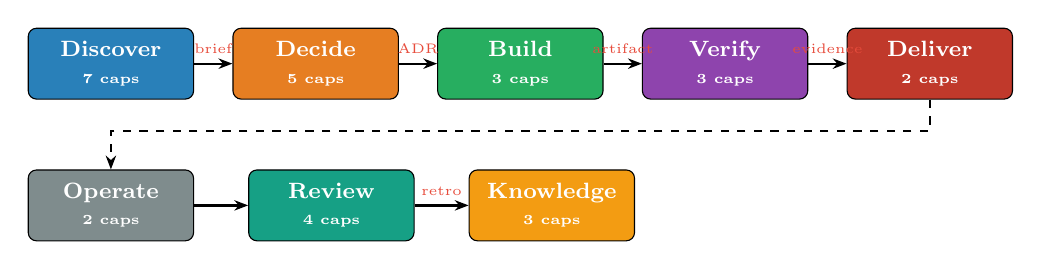
\begin{tikzpicture}[
  stage/.style={draw, rounded corners=3pt, minimum width=2.1cm, minimum height=0.9cm, align=center, font=\footnotesize\bfseries, text=white},
  arr/.style={-{Stealth[length=5pt]}, thick},
  gate/.style={font=\tiny, text=policyred, above}
]
\node[stage, fill=discoverblue] (d1) at (0,0) {Discover\\{\tiny 7 caps}};
\node[stage, fill=decideorange] (d2) at (2.6,0) {Decide\\{\tiny 5 caps}};
\node[stage, fill=buildgreen] (d3) at (5.2,0) {Build\\{\tiny 3 caps}};
\node[stage, fill=verifypurple] (d4) at (7.8,0) {Verify\\{\tiny 3 caps}};
\node[stage, fill=deliverred] (d5) at (10.4,0) {Deliver\\{\tiny 2 caps}};
\node[stage, fill=operategray] (d6) at (0,-1.8) {Operate\\{\tiny 2 caps}};
\node[stage, fill=reviewteal] (d7) at (2.8,-1.8) {Review\\{\tiny 4 caps}};
\node[stage, fill=knowledgegold] (d8) at (5.6,-1.8) {Knowledge\\{\tiny 3 caps}};

\draw[arr] (d1) -- (d2) node[gate, midway] {brief};
\draw[arr] (d2) -- (d3) node[gate, midway] {ADR};
\draw[arr] (d3) -- (d4) node[gate, midway] {artifact};
\draw[arr] (d4) -- (d5) node[gate, midway] {evidence};
\draw[arr, dashed] (d5.south) -- ++(0,-0.4) -| (d6.north);
\draw[arr] (d6) -- (d7);
\draw[arr] (d7) -- (d8) node[gate, midway] {retro};
\end{tikzpicture}
\caption{8 阶段生命周期与门控制品}
\label{fig:lifecycle}
\end{figure}

\subsection{目录结构}

系统采用\textbf{隐藏设计}——以 \texttt{\_} 前缀开头的目录不会被 Claude Code 自动发现,只有 4 个 L0 命令目录可被自动索引:

\begin{lstlisting}[language={},title={skills/ 目录布局}]
skills/
  meta/                    # L0: 系统自维护 (VISIBLE)
  build/                   # L0: 创建技能   (VISIBLE)
  research/                # L0: 科研流程   (VISIBLE)
  improve/                 # L0: 改进制品   (VISIBLE)
  _stages/                 # L2: 8 个生命周期阶段 (HIDDEN)
    discover/ decide/ build/ verify/
    deliver/ operate/ review/ knowledge/
  _paths/                  # L1: 路径模板 YAML (HIDDEN)
  _policies/               # 横切策略规则 (HIDDEN)
  _resolver/               # 解析器 + 治理文件 (HIDDEN)
  _tools/                  # 域工具族 (HIDDEN)
  _standards/              # 治理标准 (HIDDEN)
skills-registry.yaml       # 主注册表
\end{lstlisting}

\subsection{解析流程}

用户输入到最终执行的完整路径:

\begin{enumerate}[leftmargin=2em]
  \item \textbf{L0 关键词匹配}——用户输入触发某个 L0 命令(如 \texttt{/research new})
  \item \textbf{L1 路径选择}——L0 内部路由表选择对应的路径模板(如 \texttt{path-research-new-experiment})
  \item \textbf{解析器展开}——Resolver 读取路径 YAML,逐步解析每个 \texttt{capabilities\_needed}
  \item \textbf{能力索引查找}——在 \texttt{capability-index.yaml} 中找到 \texttt{cap-*} 对应的 block 文件
  \item \textbf{策略注入}——根据 step 的 \texttt{output\_type},从 \texttt{\_policies/} 注入匹配的质量规则
  \item \textbf{合约校验}——验证输入类型可用、前置条件满足
  \item \textbf{执行 + 记录}——生成 \texttt{run-*} 执行记录
\end{enumerate}

%% ============================================================
\section{核心组件}
%% ============================================================

\subsection{L0 入口命令}

系统提供 4 个用户可调用的 L0 命令,分为\textbf{系统命令}和\textbf{用户命令}两类:

\begin{table}[H]
\centering
\caption{L0 入口命令一览}
\label{tab:l0}
\begin{tabular}{llccl}
\toprule
\textbf{命令} & \textbf{类型} & \textbf{子命令数} & \textbf{路径数} & \textbf{职责} \\
\midrule
\texttt{/meta} & 系统 & 4 & 4 & 技能系统自维护与演化 \\
\texttt{/build} & 用户 & 3 types & 1 & 创建新的 L1/L2/规则 \\
\texttt{/research} & 用户 & 3 & 2 & 科研全生命周期管理 \\
\texttt{/improve} & 用户 & 2 modes & 2 & 改进现有制品 \\
\bottomrule
\end{tabular}
\end{table}

\subsubsection{/meta — 系统自维护}

\texttt{/meta} 是唯一作用于\textbf{技能架构本身}(而非用户制品)的命令,提供 4 个子命令:

\begin{itemize}[leftmargin=2em]
  \item \texttt{health} $\to$ \texttt{path-general-skill-health}(12 步)——6 维度健康扫描:命名、合约、注册表、部署、覆盖率、去重
  \item \texttt{cleanup} $\to$ \texttt{path-general-entropy-cleanup}(11 步)——9 点一致性检查 + 自动修复
  \item \texttt{quality <skill>} $\to$ \texttt{path-general-skill-quality}(11 步)——审计目标技能是否符合 skill-creator-standard
  \item \texttt{gaps} $\to$ \texttt{path-general-capability-gap}(9 步)——能力缺口诊断 $\to$ 自动构建
\end{itemize}

\begin{warningbox}[title=安全保证]
所有 \texttt{/meta} 操作遵循 PAUSE-before-action 模式——分析完成后必须等待用户确认才执行变更。评审循环最多 3 次迭代,无进展则停止。
\end{warningbox}

\subsubsection{/build — 创建新技能}

\texttt{/build} 负责在 3 层架构中创建新的构建块:

\begin{table}[H]
\centering
\begin{tabular}{lll}
\toprule
\textbf{创建类型} & \textbf{命名模式} & \textbf{放置位置} \\
\midrule
L1 路径 & \texttt{path-<domain>-<outcome>.yaml} & \texttt{\_paths/} \\
L2 能力 & \texttt{cap-<verb>-<object>.md} & \texttt{\_stages/<stage>/sub/} \\
策略规则 & \texttt{rule-<scope>-<intent>.yaml} & \texttt{\_policies/} \\
\bottomrule
\end{tabular}
\end{table}

工作流:\texttt{解析意图 $\to$ [调研] $\to$ PAUSE $\to$ 脚手架 $\to$ 实现 $\to$ 验证 $\to$ 知识沉淀}

\subsubsection{/research — 科研流程}

\texttt{/research} 管理从研究问题到知识卡片的全生命周期:

\begin{itemize}[leftmargin=2em]
  \item \texttt{new} $\to$ \texttt{path-research-new-experiment}(6 步)——结构化立项:RQ $\to$ 问题树 $\to$ 假设 $\to$ 指标 $\to$ 路线图 $\to$ 脚手架
  \item \texttt{full} $\to$ \texttt{path-research-hypothesis-to-evidence}(24 步)——完整循环:Discover $\to$ Decide $\to$ Build $\to$ Verify $\to$ Review $\to$ Knowledge
  \item \texttt{card} ——知识合成:回顾 $\to$ 原则提取 $\to$ 知识卡片 $\to$ Hub 同步
\end{itemize}

\subsubsection{/improve — 改进制品}

\texttt{/improve} 对现有代码、文档、报告进行研究驱动的改进:

\begin{itemize}[leftmargin=2em]
  \item \texttt{loop}(默认)$\to$ \texttt{path-general-improve-loop}(9 步)——研究最佳实践 $\to$ 差距分析 $\to$ 改进 $\to$ 评审循环
  \item \texttt{ratchet} $\to$ \texttt{path-general-ratchet-loop}(5 步)——检查 $\to$ 修复 $\to$ 重新检查(最多 5 次迭代)
\end{itemize}

\subsection{L1 路径模板}

8 条路径模板是系统的\textbf{编排层},每条定义了步骤序列、分支逻辑、停止规则和完成守卫:

\begin{table}[H]
\centering
\caption{8 条 L1 路径模板}
\label{tab:paths}
\small
\begin{tabular}{p{5.5cm}ccp{4.5cm}}
\toprule
\textbf{路径 ID} & \textbf{步骤数} & \textbf{所属 L0} & \textbf{职责} \\
\midrule
\texttt{path-general-skill-health} & 12 & /meta & 6 维度健康扫描 \\
\texttt{path-general-skill-quality} & 11 & /meta & 技能质量审计 \\
\texttt{path-general-entropy-cleanup} & 11 & /meta & 熵清理 + 一致性修复 \\
\texttt{path-general-capability-gap} & 9 & /meta & 能力缺口诊断与填补 \\
\texttt{path-general-improve-loop} & 9 & /improve & 研究驱动改进循环 \\
\texttt{path-general-ratchet-loop} & 5 & /improve & 轻量级棘轮修复 \\
\texttt{path-research-new-experiment} & 6 & /research & 实验立项规划 \\
\texttt{path-research-hypothesis-to-evidence} & 24 & /research & 假设到证据全循环 \\
\bottomrule
\end{tabular}
\end{table}

每条路径模板的 YAML 结构包含:

\begin{lstlisting}[language={},title={路径模板结构示例}]
id: path-<domain>-<outcome>
steps:
  - stage: discover
    capabilities_needed: [cap-intake-brief, cap-extract-brief]
    output_type: brief
    gate_requires: [intake-manifest]
applicable_policies:
  required: [rule-quality-deliverable-minimum]
  recommended: [rule-completion-guard]
stop_rules:
  max_iterations: 3
  pass_criteria: "avg_score >= 4.0"
completion_guard:
  required_evidence: [evidence-bundle, improvement-log]
\end{lstlisting}

\subsection{L2 原子能力}

29 个原子能力分布在 8 个生命周期阶段中,每个都有独立的合约声明:

\begin{table}[H]
\centering
\caption{L2 原子能力按阶段分布}
\label{tab:caps-by-stage}
\small
\begin{tabular}{lcp{8.5cm}}
\toprule
\textbf{阶段} & \textbf{数量} & \textbf{能力列表} \\
\midrule
\textcolor{discoverblue}{\textbf{Discover}} & 7 &
  \texttt{cap-intake-brief}, \texttt{cap-extract-brief}, \texttt{cap-extract-requirements}, \texttt{cap-map-problem-tree}, \texttt{cap-map-hypothesis-tree}, \texttt{cap-extract-metrics-contract}, \texttt{cap-extract-standards-scout} \\
\midrule
\textcolor{decideorange}{\textbf{Decide}} & 5 &
  \texttt{cap-compare-option-matrix}, \texttt{cap-decide-adr}, \texttt{cap-plan-exec-plan}, \texttt{cap-plan-roadmap}, \texttt{cap-plan-experiment-design} \\
\midrule
\textcolor{buildgreen}{\textbf{Build}} & 3 &
  \texttt{cap-map-tasks}, \texttt{cap-scaffold-experiment}, \texttt{cap-build-implementation} \\
\midrule
\textcolor{verifypurple}{\textbf{Verify}} & 3 &
  \texttt{cap-plan-test}, \texttt{cap-assemble-evidence-bundle}, \texttt{cap-decide-quality-gate} \\
\midrule
\textcolor{deliverred}{\textbf{Deliver}} & 2 &
  \texttt{cap-package-output}, \texttt{cap-publish-release} \\
\midrule
\textcolor{operategray}{\textbf{Operate}} & 2 &
  \texttt{cap-build-runbook}, \texttt{cap-build-observability} \\
\midrule
\textcolor{reviewteal}{\textbf{Review}} & 4 &
  \texttt{cap-review-improvement}, \texttt{cap-decide-gate}, \texttt{cap-extract-retro}, \texttt{cap-extract-design-principles} \\
\midrule
\textcolor{knowledgegold}{\textbf{Knowledge}} & 3 &
  \texttt{cap-capture-card}, \texttt{cap-sync-hub}, \texttt{cap-sync-index} \\
\midrule
\textbf{合计} & \textbf{29} & \\
\bottomrule
\end{tabular}
\end{table}

\subsubsection{能力合约结构}

每个 L2 能力以 Markdown 文件实现,头部包含 YAML 前置声明:

\begin{lstlisting}[language={},title={L2 能力合约示例 (cap-intake-brief)}]
---
cap_id: cap-intake-brief
verb: intake
object: brief
stage: discover
inputs:
  - goal-statement
  - url | file-path | repo-url
outputs:
  - intake-manifest
preconditions: []
side_effects:
  - "writes: artifacts/intake-manifest.md"
failure_modes:
  - "source_unreachable: URL or repo unavailable"
  - "ambiguous_goal: goal too vague to extract brief"
leveling: G3-V0-P2-M3
---
\end{lstlisting}

\subsection{横切策略}

9 条策略以声明式 YAML 定义,由解析器根据制品类型自动注入到门控点:

\begin{table}[H]
\centering
\caption{9 条质量策略}
\label{tab:policies}
\small
\begin{tabular}{p{5cm}p{2cm}p{6cm}}
\toprule
\textbf{策略 ID} & \textbf{触发条件} & \textbf{检查项} \\
\midrule
\texttt{rule-quality-deliverable-minimum} & 所有输出 & 证据包存在、非空、可复现 \\
\texttt{rule-completion-guard} & 横切 & 所有步骤执行、证据存在、PASS \\
\texttt{rule-improve-verify-result} & 改进日志 & 标准包($\geq$3 源)、选项矩阵、无回归 \\
\texttt{rule-skill-build-gate} & 技能制品 & 命名规范、合约有效、注册表 \\
\texttt{rule-skill-health-gate} & 健康仪表板 & 6 维度评分、阈值标准 \\
\texttt{rule-entropy-cleanup-gate} & 熵报告 & 确定性验证、幽灵引用检测 \\
\texttt{rule-capability-gap-detection} & 缺口分析 & 分类、影响$\times$工作量评分 \\
\texttt{rule-research-front-loading} & 科研制品 & 假设驱动、指标合约、止损规则 \\
\texttt{rule-layer-dependency} & 所有路径 & 层间依赖合规(无跨层捷径) \\
\bottomrule
\end{tabular}
\end{table}

%% ============================================================
\section{治理机制}
%% ============================================================

\subsection{命名治理}

系统通过\textbf{受控词汇表}强制执行一致的命名:

\subsubsection{18 受控动词}

所有 L2 能力的动词必须来自以下受控表:

\begin{multicols}{3}
\begin{enumerate}[leftmargin=1.5em, itemsep=0pt]
  \item \texttt{intake}
  \item \texttt{extract}
  \item \texttt{map}
  \item \texttt{compare}
  \item \texttt{decide}
  \item \texttt{plan}
  \item \texttt{scaffold}
  \item \texttt{build}
  \item \texttt{render}
  \item \texttt{assemble}
  \item \texttt{package}
  \item \texttt{publish}
  \item \texttt{check}
  \item \texttt{track}
  \item \texttt{triage}
  \item \texttt{review}
  \item \texttt{capture}
  \item \texttt{sync}
\end{enumerate}
\end{multicols}

每个动词定义了别名(用户同义词)和阶段边界(哪些阶段可以使用该动词)。

\subsubsection{91 规范对象}

对象表定义了所有合法的能力对象名,按领域分组(research、paper、repo、webui、docs 等),每个对象有 \texttt{used\_in} 引用。

\subsubsection{命名规则}

\begin{table}[H]
\centering
\begin{tabular}{lll}
\toprule
\textbf{层} & \textbf{模式} & \textbf{示例} \\
\midrule
L2 能力 & \texttt{cap-<verb>-<object>} & \texttt{cap-intake-brief} \\
L1 路径 & \texttt{path-<domain>-<outcome>} & \texttt{path-research-new-experiment} \\
策略 & \texttt{rule-<scope>-<intent>} & \texttt{rule-quality-deliverable-minimum} \\
执行记录 & \texttt{run-<path>-<ctx>-<date>-<seq>} & \texttt{run-path-research-...-20260224-01} \\
\bottomrule
\end{tabular}
\end{table}

\textbf{检查规则}:kebab-case only $|$ 3--6 token $|$ 动词必须来自受控表 $|$ 对象必须来自规范表 $|$ 正确前缀

\subsection{制品类型系统}

\texttt{artifact-types.yaml} 定义了 130 种制品类型,涵盖:

\begin{itemize}[leftmargin=2em]
  \item \textbf{原始输入}:\texttt{goal-statement}, \texttt{url}, \texttt{file-path}, \texttt{repo-url}
  \item \textbf{阶段输出}:\texttt{brief}, \texttt{intake-manifest}, \texttt{adr}, \texttt{evidence-bundle}, \texttt{knowledge-card}
  \item \textbf{横切制品}:\texttt{improvement-log}, \texttt{entropy-report}, \texttt{health-dashboard}
\end{itemize}

制品类型用于解析器的\textbf{类型兼容性验证}——步骤 $n$ 的输出必须满足步骤 $n+1$ 的输入要求。

\subsection{等级系统(Leveling)}

每个能力标记一个 \texttt{Gx-Vy-Pz-Mk} 标签,用于解析器排序和系统健康评估:

\begin{table}[H]
\centering
\begin{tabular}{llp{7cm}}
\toprule
\textbf{维度} & \textbf{范围} & \textbf{含义} \\
\midrule
G (通用性) & G0--G3 & G0=临时 $\to$ G3=核心跨域 \\
V (易变性) & V0--V3 & V0=稳定 $\to$ V3=快速变化 \\
P (成熟度) & P0--P3 & P0=草稿 $\to$ P3=硬化 \\
M (观测度) & M0--M4 & M0=存根 $\to$ M4=生产验证 \\
\bottomrule
\end{tabular}
\end{table}

核心能力的典型等级为 \texttt{G3-V0-P2-M3}(核心、稳定、生产就绪、已观测使用)。

%% ============================================================
\section{解析器机制}
%% ============================================================

\subsection{解析算法}

解析器(\texttt{\_resolver/resolver.md})执行 7 步解析流程:

\begin{enumerate}[leftmargin=2em]
  \item \textbf{加载路径模板}——读取 \texttt{\_paths/<path\_id>.yaml},验证结构完整性
  \item \textbf{逐步解析}——对每个步骤:
    \begin{enumerate}[label=\alph*.]
      \item 在 \texttt{capability-index.yaml} 中查找 \texttt{cap\_id}
      \item 验证动词来自 \texttt{verbs.yaml},对象来自 \texttt{objects.yaml}
      \item 如果精确匹配失败,启动\textbf{模糊搜索}
      \item 多提供者时按 P/M 等级排序
    \end{enumerate}
  \item \textbf{模糊搜索}(降级查找)——按动词+对象模式 $\to$ 按输出类型 $\to$ 按输入类型 $\to$ 按阶段
  \item \textbf{加载策略}——\texttt{required} 策略必须注入,\texttt{recommended} 按上下文注入
  \item \textbf{插入策略检查}——匹配策略的 \texttt{triggers.output\_types} 与步骤的 \texttt{output\_type}
  \item \textbf{生成执行 ID}——格式:\texttt{run-<path>-<ctx>-<yyyymmdd>-<seq>}
  \item \textbf{返回解析后的执行计划}
\end{enumerate}

\subsection{治理文件}

解析器依赖 5 个治理文件:

\begin{table}[H]
\centering
\begin{tabular}{lcp{7cm}}
\toprule
\textbf{文件} & \textbf{条目数} & \textbf{职责} \\
\midrule
\texttt{verbs.yaml} & 18 & 受控动词 + 别名 + 阶段边界 \\
\texttt{objects.yaml} & 91 & 规范对象 + 领域标签 + 引用 \\
\texttt{artifact-types.yaml} & 130 & 制品类型定义(输入/输出) \\
\texttt{capability-index.yaml} & 29 & cap-* $\to$ block 文件映射 \\
\texttt{resolver.md} & — & 解析算法规范 \\
\bottomrule
\end{tabular}
\end{table}

%% ============================================================
\section{关键设计模式}
%% ============================================================

\subsection{门控检查工作流}

每条路径在关键动作前设置显式门控:

\begin{itemize}[leftmargin=2em]
  \item \textbf{PAUSE 点}——分析完成后等待用户确认方向
  \item \textbf{Verify 步骤}——必须 PASS 才能继续
  \item \textbf{Critic 循环}——迭代直到 PASS 或预算耗尽
  \item \textbf{Completion Guard}——强制所有步骤完成
\end{itemize}

\begin{infobox}[title=完成守卫机制]
\texttt{rule-completion-guard} 通过状态文件 \texttt{.claude/completion-guard.local.md} 追踪执行进度。当且仅当所有步骤完成、所有证据存在、验证通过时,输出 \texttt{<promise>ALL\_STEPS\_COMPLETE</promise>} 信号。
\end{infobox}

\subsection{多分支路径}

路径支持条件分支:

\begin{itemize}[leftmargin=2em]
  \item \texttt{decision-gate} $\to$ ``continue''(循环)/ ``change direction''(转向)/ ``publish''(外部发布)
  \item \texttt{quality-gate} $\to$ ``PASS'' / ``FAIL''(重试)
  \item \texttt{critic-review} $\to$ ``ITERATE''(循环)/ ``PASS''(完成)/ ``BUDGET\_EXHAUSTED''(停止)
\end{itemize}

\subsection{组合优于继承}

系统采用扁平组合模式而非层次继承:

\begin{itemize}[leftmargin=2em]
  \item 每个 L2 能力是独立的——可以单独运行
  \item L1 路径通过编排组合 L2 能力
  \item 策略环绕在步骤周围(不嵌入能力内部)
  \item L0 命令是薄路由器(逻辑在路径中,不在命令中)
\end{itemize}

\subsection{扩展点设计}

在 \texttt{path-research-hypothesis-to-evidence} 中预留了领域扩展点:

\begin{table}[H]
\centering
\small
\begin{tabular}{ll}
\toprule
\textbf{扩展能力 ID} & \textbf{用途} \\
\midrule
\texttt{cap-build-data-pipeline} & 领域特定数据处理 \\
\texttt{cap-build-model-loss} & 模型架构定义 \\
\texttt{cap-render-eval-harness} & 评估脚本生成 \\
\texttt{cap-track-experiment} & 实验自动记录 \\
\texttt{cap-check-metric-sanity} & 指标鲁棒性检查 \\
\texttt{cap-check-reproducibility} & 可复现性验证 \\
\texttt{cap-plan-resource-budget} & 计算资源预算 \\
\bottomrule
\end{tabular}
\end{table}

这些扩展点由私有仓库实现,核心模块不包含它们的具体实现。

%% ============================================================
\section{部署模型}
%% ============================================================

\subsection{部署脚本}

\texttt{tools/setup.sh} 将 meta-skills 部署到 \texttt{\textasciitilde/.claude/skills/},供 Claude Code 使用:

\begin{enumerate}[leftmargin=2em]
  \item 复制 4 个 L0 命令目录(使用 \texttt{cp -rL} 解引用符号链接)
  \item 复制 8 个生命周期阶段(\texttt{\_stages/})
  \item 复制架构层(\texttt{\_paths/}, \texttt{\_policies/}, \texttt{\_resolver/}, \texttt{\_standards/})
  \item 创建符号链接(\texttt{\_tools/}, \texttt{skills-registry.yaml})
  \item 验证部署完整性(检查文件存在、计数)
\end{enumerate}

\begin{warningbox}[title=关键限制]
Claude Code \textbf{无法}通过符号链接发现 SKILL.md 文件。解决方案:对技能目录使用 \texttt{cp -rL}(解引用复制),仅 \texttt{\_tools/} 和 \texttt{skills-registry.yaml} 保留为符号链接。
\end{warningbox}

\subsection{子模块集成}

Meta-Skills 设计为 Git submodule 使用:

\begin{lstlisting}[language=bash,title={子模块集成方式}]
# 添加为子模块
git submodule add <url> meta-skills

# 私有仓库的 setup.sh 应:
# 1. 先部署核心(bash meta-skills/tools/setup.sh)
# 2. 覆盖领域扩展(复制额外的 L0/L1/L2)
# 3. 使用扩展的解析器(verbs/objects 是核心的超集)
\end{lstlisting}

\subsection{验证工具}

系统提供 4 个验证脚本:

\begin{table}[H]
\centering
\begin{tabular}{lcp{6.5cm}}
\toprule
\textbf{工具} & \textbf{行数} & \textbf{职责} \\
\midrule
\texttt{setup.sh} & 120 & 部署到 \textasciitilde/.claude/skills/ \\
\texttt{build\_capability\_index.sh} & 92 & 从 block 文件重建 capability-index \\
\texttt{validate\_contracts.sh} & 172 & 验证 YAML 前置合约 \\
\texttt{validate\_aliases.sh} & 149 & 验证触发词 + 能力引用 \\
\bottomrule
\end{tabular}
\end{table}

%% ============================================================
\section{定量分析}
%% ============================================================

\subsection{系统规模统计}

\begin{table}[H]
\centering
\caption{Meta-Skills 系统规模}
\label{tab:stats}
\begin{tabular}{llr}
\toprule
\textbf{类别} & \textbf{说明} & \textbf{数量} \\
\midrule
L0 入口命令 & 用户直接调用 & 4 \\
L1 路径模板 & 多步骤编排 & 8 \\
L2 原子能力 & 构建块 & 29 \\
横切策略 & 质量门禁 & 9 \\
受控动词 & 命名治理 & 18 \\
规范对象 & 命名治理 & 91 \\
制品类型 & 合约系统 & 130 \\
部署脚本 & 工具链 & 4 \\
\midrule
\textbf{治理密度} & 策略 / 能力 & 0.31 \\
\textbf{编排比} & 路径步骤 / 能力 & 2.90 \\
\textbf{词汇覆盖} & 动词 $\times$ 对象 & 1,638 \\
\bottomrule
\end{tabular}
\end{table}

\subsection{阶段覆盖分析}

\begin{figure}[H]
\centering
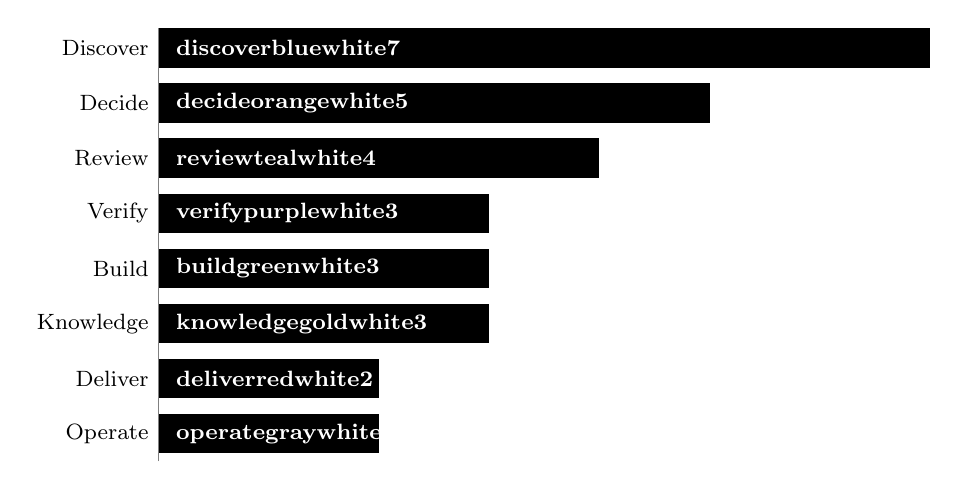
\begin{tikzpicture}
\begin{scope}
  \foreach \stage/\count/\color/\ypos in {
    Discover/7/discoverblue/7,
    Decide/5/decideorange/6,
    Review/4/reviewteal/5,
    Verify/3/verifypurple/4,
    Build/3/buildgreen/3,
    Knowledge/3/knowledgegold/2,
    Deliver/2/deliverred/1,
    Operate/2/operategray/0
  } {
    \fill[\color!70] (0,\ypos*0.7) rectangle (\count*1.4, \ypos*0.7+0.5);
    \node[left, font=\footnotesize] at (0, \ypos*0.7+0.25) {\stage};
    \node[right, font=\footnotesize\bfseries, text=white] at (0.1, \ypos*0.7+0.25) {\count};
  }
  \draw[thin, gray] (0,-0.1) -- (0,5.4);
\end{scope}
\end{tikzpicture}
\caption{各阶段能力覆盖数(横条图)}
\label{fig:coverage}
\end{figure}

\textbf{观察}:
\begin{itemize}[leftmargin=2em]
  \item \textbf{Discover}(7 个)覆盖最密——反映"前端加载"设计哲学(在动手前充分理解问题)
  \item \textbf{Decide}(5 个)次之——决策阶段需要多种比较和规划工具
  \item \textbf{Deliver/Operate}(各 2 个)最少——这些阶段更多依赖外部工具和域特定实现
  \item \textbf{Review}(4 个)包含评审、门控、回顾、原则提取——知识闭环的关键
\end{itemize}

\subsection{等级分布}

\begin{table}[H]
\centering
\begin{tabular}{lcc}
\toprule
\textbf{等级} & \textbf{数量} & \textbf{占比} \\
\midrule
G3-V0-P2-M3(核心稳定已验证) & 18 & 62.1\% \\
G3-V1-P2-M3(核心、微变、已验证) & 5 & 17.2\% \\
G3-V1-P1-M2(核心、微变、试点) & 2 & 6.9\% \\
G2-V1-P1-M1(多域、新建) & 2 & 6.9\% \\
G3-V0-P1-M2(核心、稳定、试点) & 1 & 3.4\% \\
G3-V0-P3-M3(核心、稳定、硬化) & 1 & 3.4\% \\
\bottomrule
\end{tabular}
\end{table}

唯一达到 P3(硬化)等级的是 \texttt{cap-decide-quality-gate}——作为质量最终裁决者,它本身需要最高的可靠性。

%% ============================================================
\section{与私有仓库的关系}
%% ============================================================

Meta-Skills 作为公开子模块,与私有仓库形成\textbf{核心-扩展}架构:

\begin{table}[H]
\centering
\caption{公开核心 vs 私有扩展}
\begin{tabular}{lcc}
\toprule
\textbf{类别} & \textbf{公开核心} & \textbf{私有扩展} \\
\midrule
L0 命令 & 4 & +8(含 workflow, office 等) \\
L1 路径 & 8 & +19 \\
L2 能力 & 29 & +40 \\
策略 & 9 & +15 \\
插件 & 0 & 11 \\
\midrule
\textbf{合计} & \textbf{50} & \textbf{+93} \\
\bottomrule
\end{tabular}
\end{table}

私有仓库通过以下方式扩展核心:
\begin{enumerate}[leftmargin=2em]
  \item 添加领域特定的 L0 命令(如 \texttt{/read}, \texttt{/write}, \texttt{/search})
  \item 实现核心预留的扩展点能力(如 \texttt{cap-build-data-pipeline})
  \item 添加领域策略(如 \texttt{rule-webui-dev-server-verify})
  \item 添加插件技能(如 docx, pdf, pptx, xlsx 等办公工具)
  \item 扩展受控词汇表(更多动词和对象)
\end{enumerate}

%% ============================================================
\section{总结}
%% ============================================================

\subsection{架构优势}

Meta-Skills 通过 3 层调用架构实现了以下目标:

\begin{enumerate}[leftmargin=2em]
  \item \textbf{简洁的用户界面}——4 个 L0 命令覆盖了系统维护(meta)、创建(build)、科研(research)、改进(improve)四大类需求
  \item \textbf{可靠的质量保证}——9 条策略自动注入到门控点,无需人工记忆检查清单
  \item \textbf{严格的命名一致性}——18 动词 $\times$ 91 对象的受控词汇表消除了命名歧义
  \item \textbf{灵活的扩展性}——公开核心 + 私有扩展的子模块模式,领域能力可独立演进
  \item \textbf{自维护能力}——\texttt{/meta} 命令让系统能诊断和修复自身的健康问题
  \item \textbf{可追溯性}——合约驱动的类型系统和执行记录确保每个决策可追溯
\end{enumerate}

\subsection{演进方向}

基于当前状态,系统的潜在演进方向包括:

\begin{itemize}[leftmargin=2em]
  \item \texttt{rule-harness-safety.yaml}——meta 操作安全护栏(已列入待办)
  \item 独立部署测试——验证公开仓库的 \texttt{setup.sh} 在全新环境下的可用性
  \item 设计手册更新——反映从 1 L0 到 4 L0 的架构升级
  \item 更多 P3(硬化)能力——当前仅 1/29 达到 P3 等级
\end{itemize}

\begin{corebox}[title=一句话总结]
Meta-Skills 是一个\textbf{合约驱动、策略注入、自维护}的 AI Agent 技能基础设施,通过 3 层分离(入口 / 编排 / 原子)+ 8 阶段生命周期 + 严格命名治理,实现了复杂 Agent 能力的可组合管理。
\end{corebox}

\end{document}
